\documentclass[landscape,twocolumn,letter]{book}
% Licencia y derechos: consulte ../../LICENSE-CC-BY-4.0.
% Las figuras y demás materiales de terceros pueden tener derechos separados y deben identificarse.

\usepackage{geometry}
\usepackage{amsmath}
\usepackage{mathrsfs}
\usepackage{graphicx}
\usepackage[utf8]{inputenc}
\usepackage{hyperref}

\usepackage[T1]{fontenc}
\usepackage{imakeidx}
\makeindex 


\title{Apuntes de Profesor}
\date{2022 Octubre\\rev 0.1k}
\author{Alberto Medrano\thanks{Instructor, Universidad de Los Andes (ULA)}}

\begin{document}
	\maketitle
	
	Saludos, éstos son de mis apuntes personales para con la materia Electrónica II, de encontrar algún error o sugerencia por favor notificar vía correo electrónico \href{mailto: ecadmaster@hotmail.com}{ ecadmaster@hotmail.com}
	
	\section{Tema I: Dispositivos Electrónicos}
	- en desarrollo -
		\subsection{LEDs}
		- pendiente en apuntes -
		
		\subsection{7-seg}
		Contiene siete diodos LED rectangulares (A hasta G). Cada LED se denomina segmento porque forma parte del carácter que se están mostrando.
		
		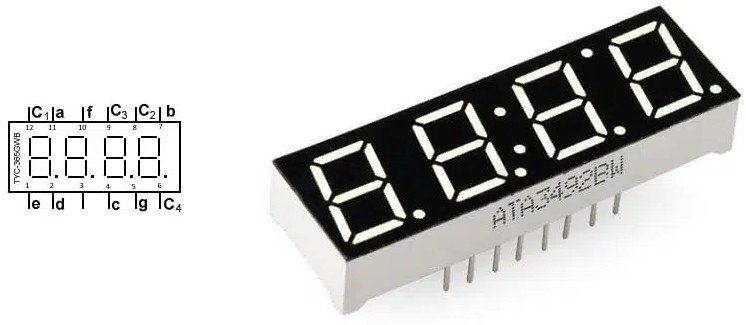
\includegraphics[width=8cm]{_fig/1d2_7seg-cc_x4.jpg}
		
		Pueden presentar en dos tipos de configuraciones: ánodo común y catodo común.
		
		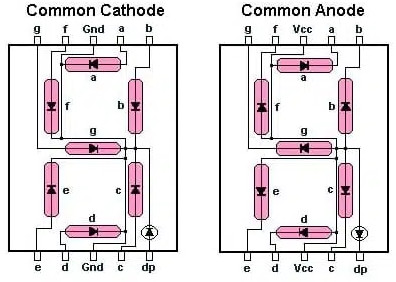
\includegraphics[width=8cm]{_fig/1d2_7seg-ca-cc.jpg}
		
		De las limitaciones los display 7-seg se recomiendo su uso para representar números y tal vez algunos caracteres del alfabeto, otras alternativas pueden ser los LED de 14-seg y 16-seg como se ve a continuación:

		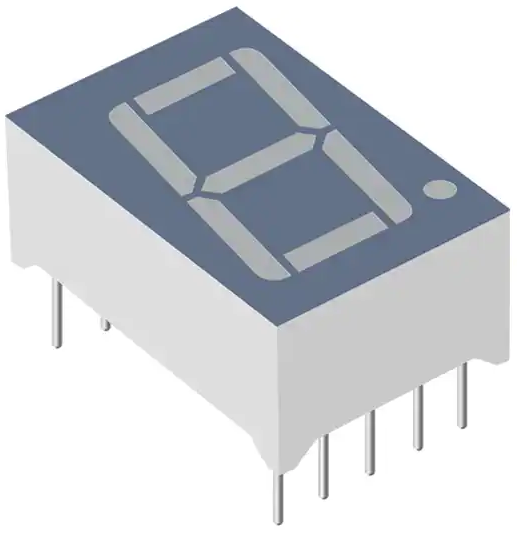
\includegraphics[width=3cm]{_fig/1d2_7seg.png}
		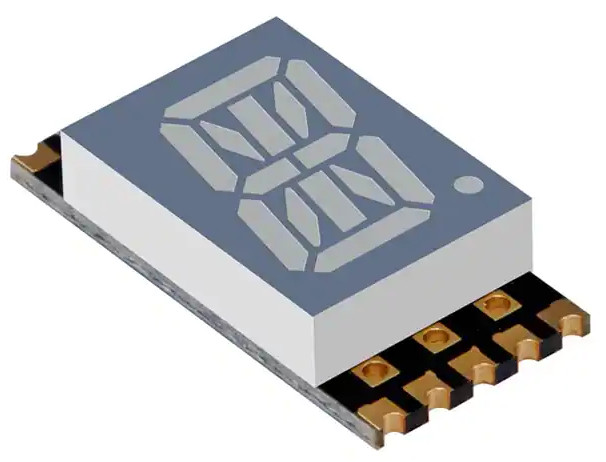
\includegraphics[width=3cm]{_fig/1d2_14seg.jpg}
		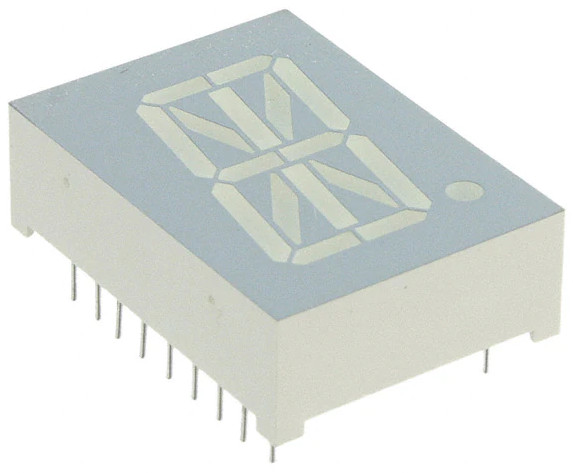
\includegraphics[width=3cm]{_fig/1d2_16seg.jpg}
		
		El uso de estos \textit{displays} con más segmentos permiten representar con más comodidad todos los caracteres del alfabeto español.
		
		\subsection{Fotorresistencias, fotodiodos}
		- pendiente en apuntes -
		
		\subsection{SCRS y TRIAC}
		El SCR (\textit{silicon controlled rectifier}, rectificador controlado por silicio) es el tiristor más utilizado. Se utiliza normalmente para conmutar corrientes muy elevadas. Para ponerlo en modo conducción es necesario aplicar una corriente y tensión en el pin Puerta/Gate $(G)$. Para bloquearlo, hay que reducir la tensión entre sus terminales ánodo/cátodo a prácticamente cero.
		
		\subsection{Criterios de selección acopladores ópticos}
		- pendiente en apuntes -
		
			\subsubsection{Optoacoplador}
			Combina un diodo LED y un fotodiodo en un mismo encapsulado. Está formado por un LED (normalmente infrarrojo) en la entrada y un fotodiodo en la salida.

			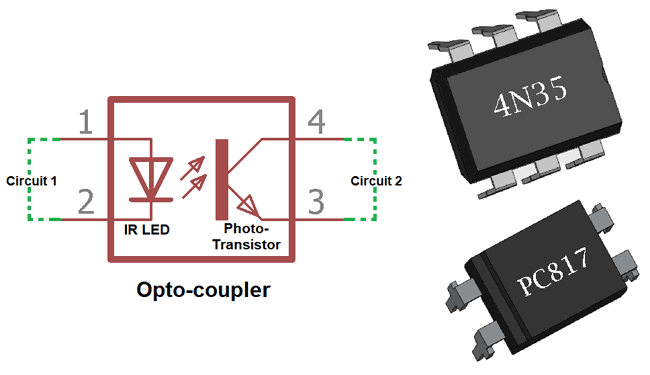
\includegraphics[width=8cm]{_fig/1d1_optocoupler.png}

	\section{Tema II: Circuitos de conmutación}
		\subsection{Circuitos lineales y no lineales}
		Varios tipos de dispositivos eléctricos se fabrican combinando elementos lineales y no lineales. Entonces, para comprender mejor el diseño básico de estos dispositivos eléctricos, debemos conocer:
		
			\subsubsection{Circuitos lineales}
			Básicamente, un circuito lineal es un circuito eléctrico y los parámetros de estos circuitos como Resistencia, Capacitancia, Inductancia, etc. son siempre constantes.
			
			Es decir, podemos decir que un circuito lineal se llama circuito que cambia los parámetros del circuito con cambios en el voltaje y la corriente.
			
			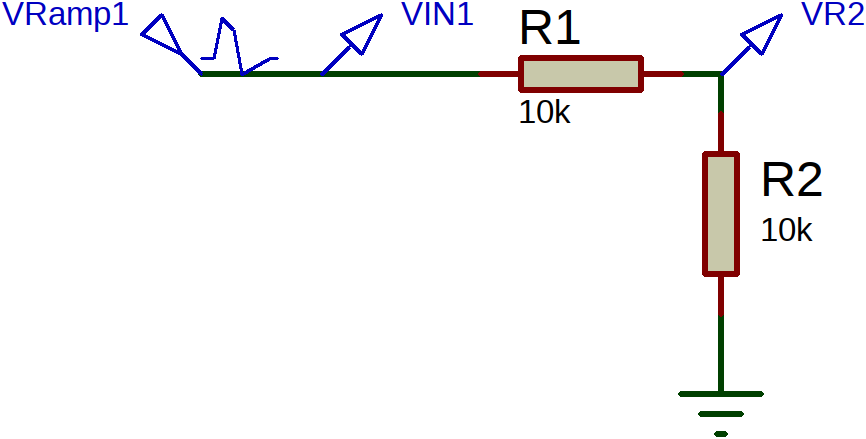
\includegraphics[width=4.5cm]{_fig/CircuitoLineal_pA.png}
			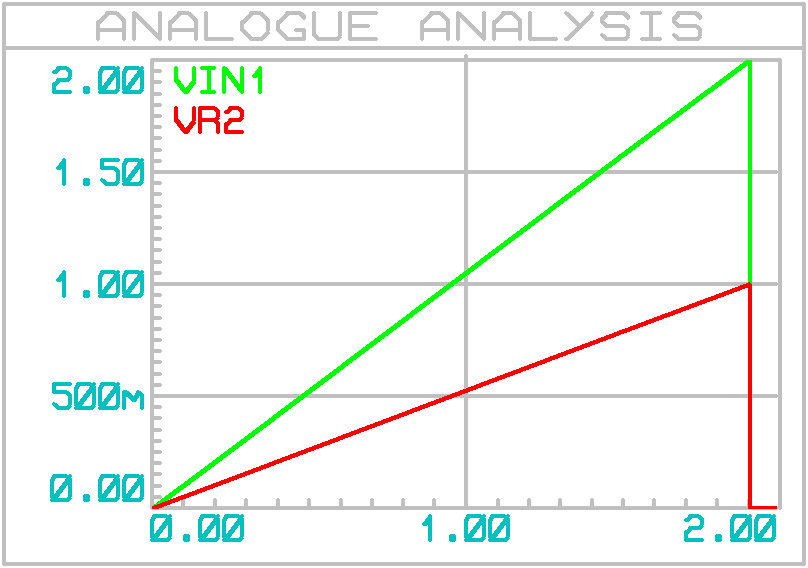
\includegraphics[width=4.5cm]{_fig/CircuitoLineal_pB.png}
			
			\subsubsection{Circuitos no lineales}
			El circuito no lineal también es un circuito eléctrico, pero el cambio de voltaje y corriente en este circuito cambia los parámetros de los circuitos, como formas de onda, resistencia, inductancia, etc.
			
			Es decir, un circuito no lineal se denomina circuito en el que el voltaje de la corriente cambia los parámetros del circuito.
			
			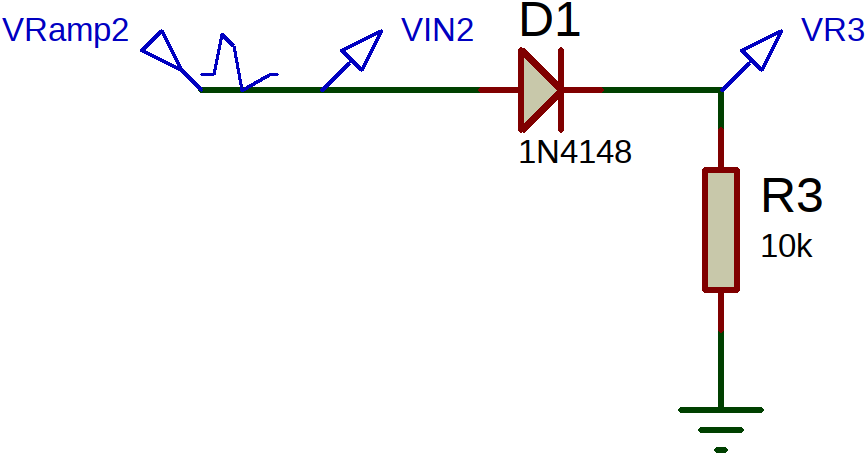
\includegraphics[width=4.5cm]{_fig/CircuitoNoLineal_pA.png}
			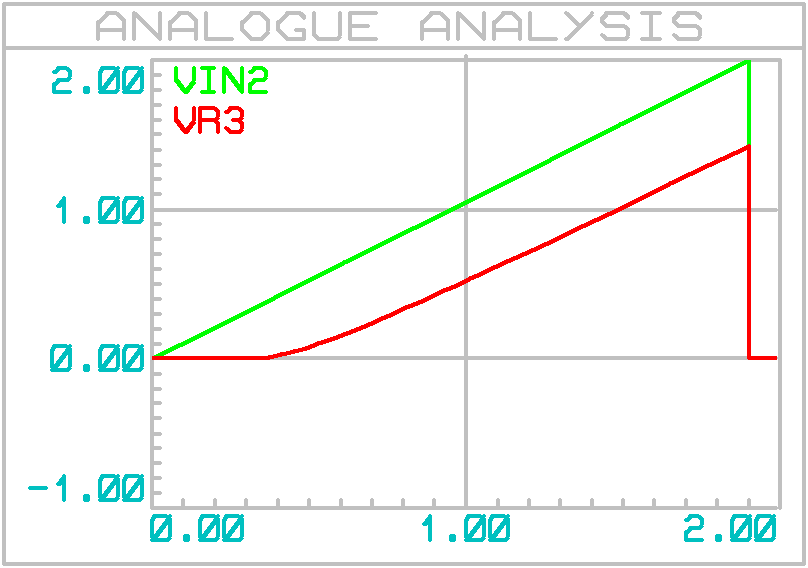
\includegraphics[width=4.5cm]{_fig/CircuitoNoLineal_pB.png}

		\subsection{Circuitos limitadores o recortadores}
		Limitador o recortador es un circuito que, mediante el uso de resistencias y diodos, permite eliminar tensiones que no nos interesen para que no lleguen a un determinado punto de un circuito.
			\subsubsection{Recortador sin polarizar}
			Es como sigue:
			
			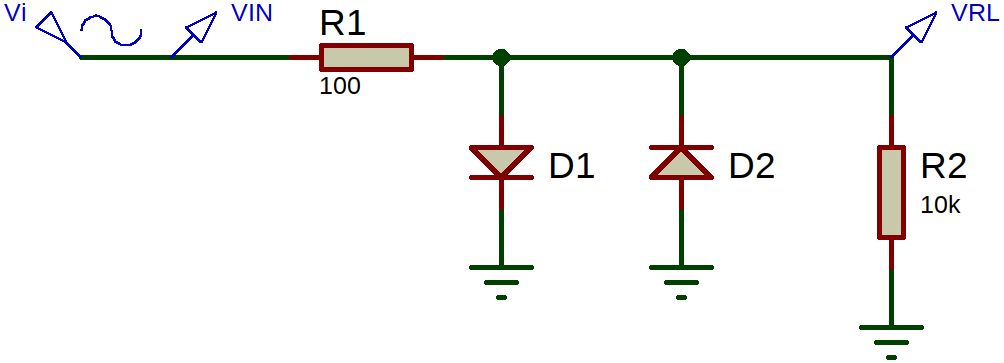
\includegraphics[width=9cm]{_fig/RecortadorSinPolarizar_pA.png}

			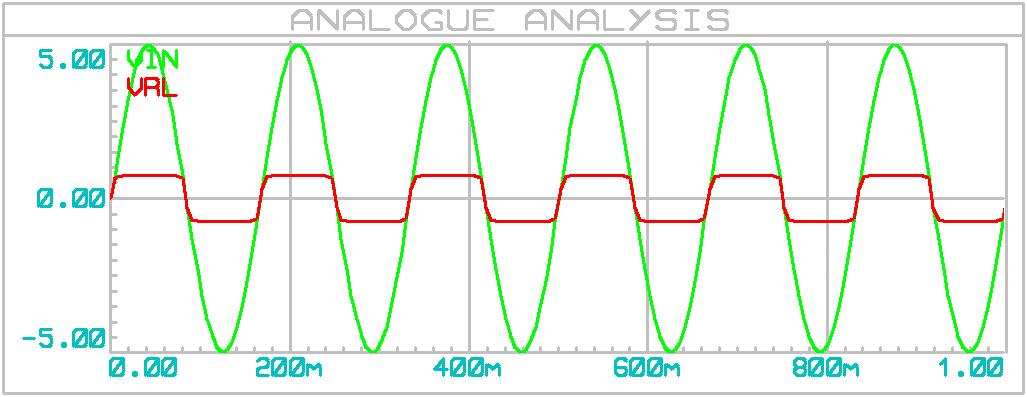
\includegraphics[width=9cm]{_fig/RecortadorSinPolarizar_pB.png}
			
			Aunque la resistencia limitadora (R1) pueda parecer innecesaria, es importante entender que en realidad es parte imprescindible del limitador, ya que si no estuviera conectada, al polarizarse uno de los diodos directamente (los dos diodos no pueden estar polarizados directamente al mismo tiempo), este comenzaría a conducir la corriente eléctrica sin control y se destruiría. Como su propio nombre indica, la resistencia limitadora tiene como función limitar la corriente que atraviesa los diodos.
			
			De este modo, si la tensión de entrada supera por cualquier motivo los $0.7V$ el diodo D1 quedará polarizado directamente y recortará el exceso de tensión. De igual forma, cuando la tensión de entrada disminuya de $-0.7V$, el diodo D2 quedará polarizado directamente y recortará el exceso de tensión que podría dañar nuestra carga.
			
			\subsubsection{Recortador polarizado}
			Muchas veces no nos interesa que los diodos limiten las tensiones de entrada a los $0.7V$ o a los $-0.7V$. Por ejemplo, puede que lo que estemos buscando es que a la entrada no le lleguen tensiones superiores a los 10V o inferiores a los $-10V$ (estas tensiones son aleatorias, nosotros elegimos las que más nos interesen), en ese caso no podemos usar el circuito antes mencionado, ahora necesitamos un limitador polarizado. La única diferencia respecto al anterior limitador es que en este caso vamos a polarizar los diodos con fuentes DC, a fin de que sea necesaria una tensión de entrada mayor que $0.7V$ para que los diodos se polaricen directamente.
			
			Si lo que buscamos es que la tensión en la carga no sea mayor de $10V$ ni inferior de $-10V$, montaremos el siguiente circuito.
			
			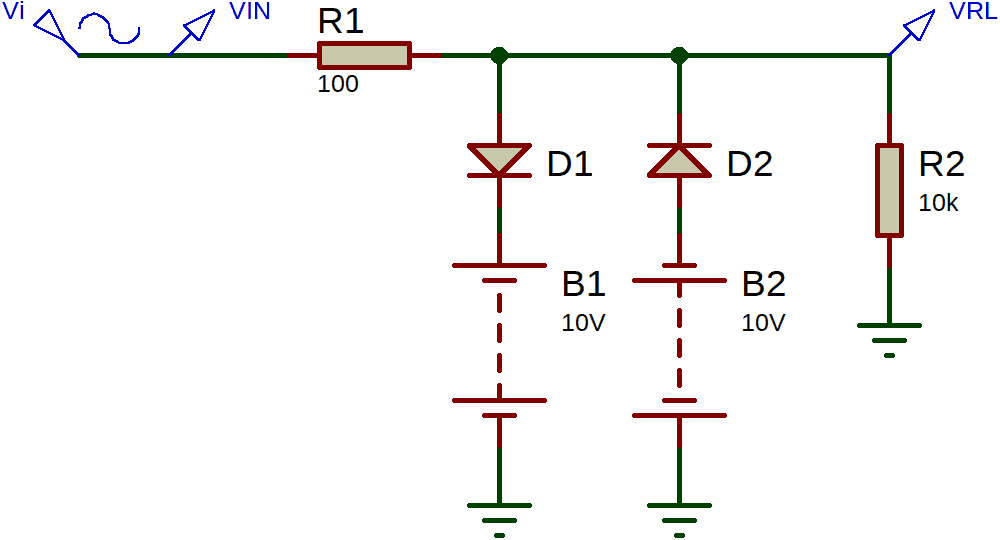
\includegraphics[width=9cm]{_fig/RecortadorPolarizado_pA.png}
			
			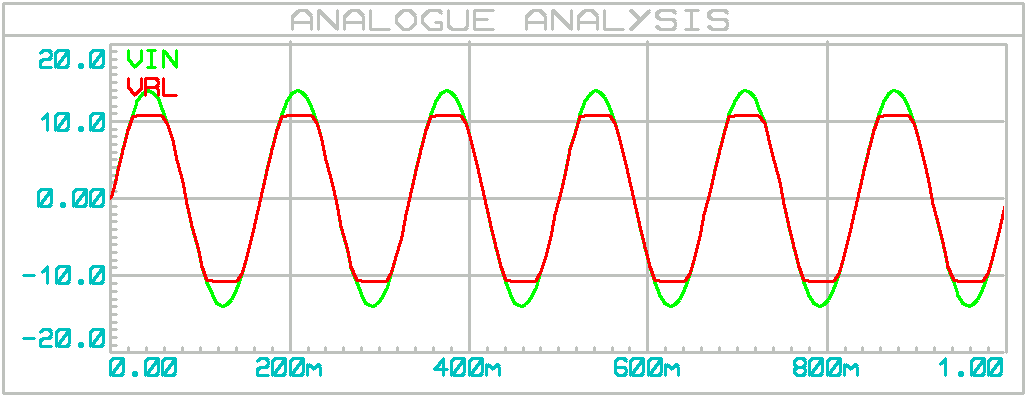
\includegraphics[width=9cm]{_fig/RecortadorPolarizado_pB.png}
						
		\subsection{Régimen transitorios circuitos RLCD}
			\subsubsection{C y L en el dominio de Laplace}
 			En régimen permanente y transitorio:
 			
 			\includegraphics[width=9cm]{_fig/Laplace_CL_Regimen_PandT.pdf}

			-- en desarrollo --
		\subsection{title}
			
	\section{Tema III: Multibrivadores, Temporizadores y Generador De Funciones}
	Un multivibrador es un circuito oscilador capaz de generar una onda cuadrada. Según su funcionamiento, los multivibradores se pueden dividir en dos clases: De funcionamiento continuo (astable) y de funcionamiento impulsado (monoestable y biestable)
		\subsection{Monoestable, astable, biestable}
			\subsubsection{Monoestable}
			Realiza una función secuencial consistente en que al recibir una excitación exterior, cambia de estado y se mantiene en él durante un periodo que viene determinado por una constante de tiempo. Transcurrido dicho período, la salida del monoestable vuelve a su estado original. Por tanto, tiene un estado estable (de aquí su nombre) y un estado casi estable.
			\subsubsection{Astable}
			Astable es un circuito multivibrador que no tiene ningún estado estable, lo que significa que posee dos estados inestables entre los que conmuta, permaneciendo en cada uno de ellos un tiempo determinado.
			\subsubsection{Biestable}
			Biestable, flip-flop y latch, es un circuito multivibrador, que tiene dos estados estables y puede almacenar información. Se puede hacer que cambie de estado mediante señales aplicadas a una o más entradas de control y tiene una o dos salidas.

		\subsection{Conceptos, ciclo de servicio}
		
		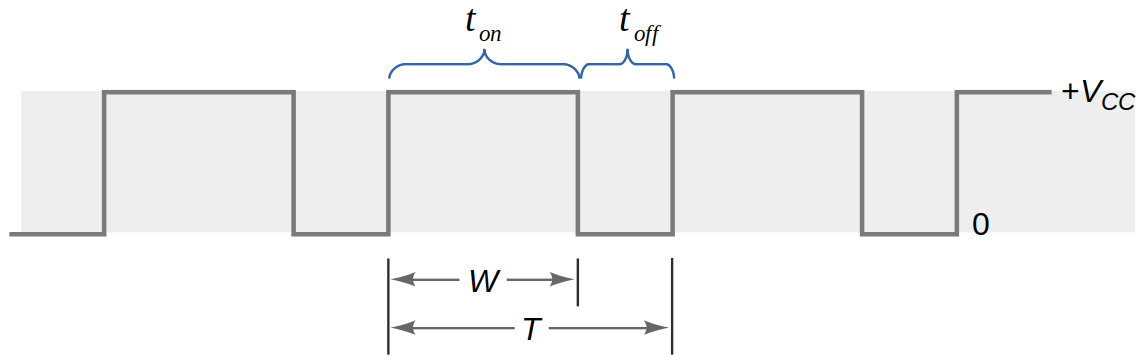
\includegraphics[width=9cm]{_fig/3d2_CicloDeServicio.png}
		
		donde:
		
		\[ t_{on} = W \]
		\[ t_{off} = T-W \]
		\[ T = t_{off} + t_{on} \]
		\[ f = 1/T \]

		\subsection{Estudio en bloque del temporizador NE555 o similar}
		Es un circuito integrado temporizador, diseñado en el año 1971 por Hans Camenzind (Analog Engineer), primera producción en 1972, si diseño original contiene: 23 transistores, 16 resistencias y 2 diodos y su esquema es como se ve en la siguiente figura:
		
		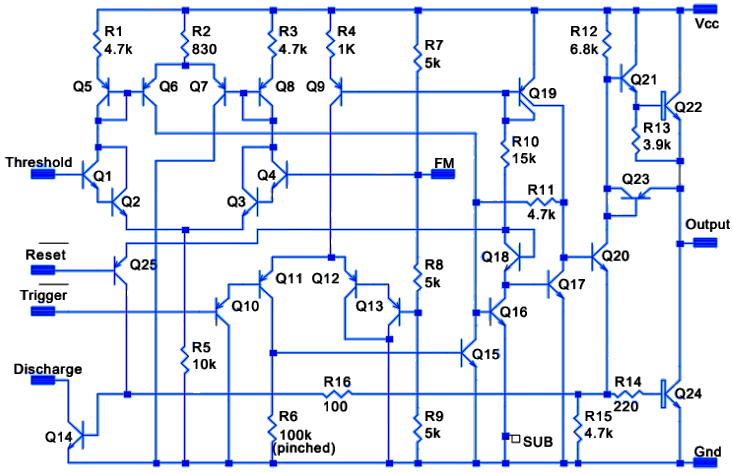
\includegraphics[width=9cm]{_fig/3d3_555-schematic.png}
		
		Componente aún activo (en producción) puede presentarse en varios encapsulados y variantes:
		
		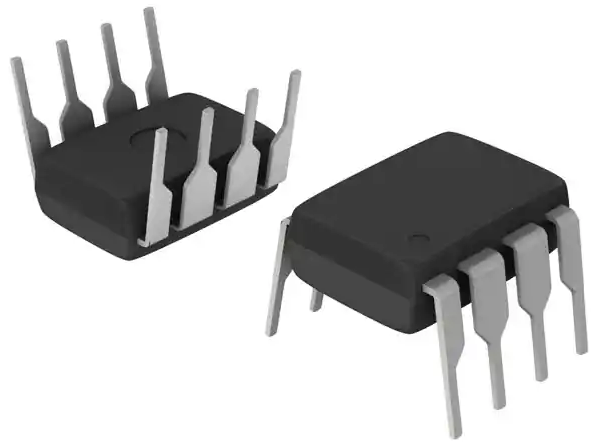
\includegraphics[width=1.7cm]{_fig/3d3_555_8-DIP.png}
		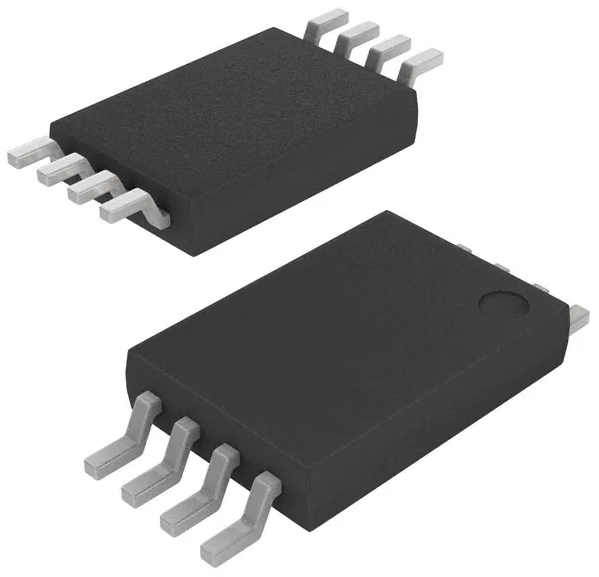
\includegraphics[width=1.7cm]{_fig/3d3_555_8-TSSOP.png}
		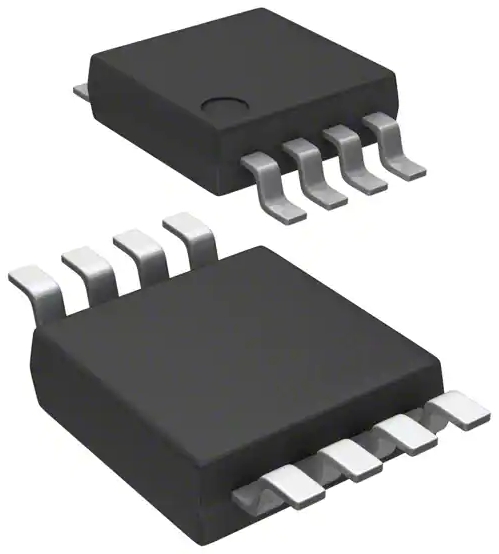
\includegraphics[width=1.7cm]{_fig/3d3_555_MSOP-8.png}
		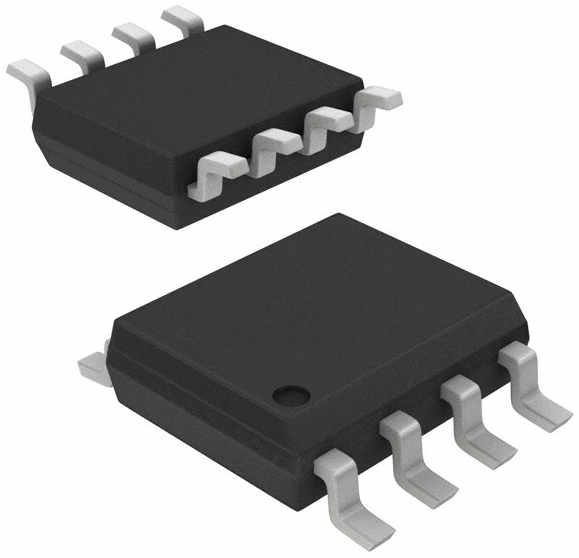
\includegraphics[width=1.7cm]{_fig/3d3_555_SOIC-8.png}
		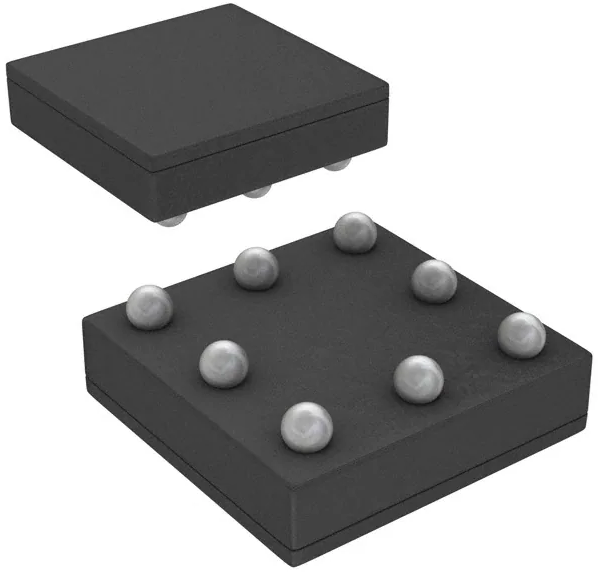
\includegraphics[width=1.7cm]{_fig/3d3_555_TPA08EFA}

		También existen variantes con nombre similar, 556 y 558 contiene 2 y 4 bloques completos del 555 original permitiendo configurar múltiples temporizadores con un IC simple.
		
		\subsubsection{Configuración Monoestable}
		
		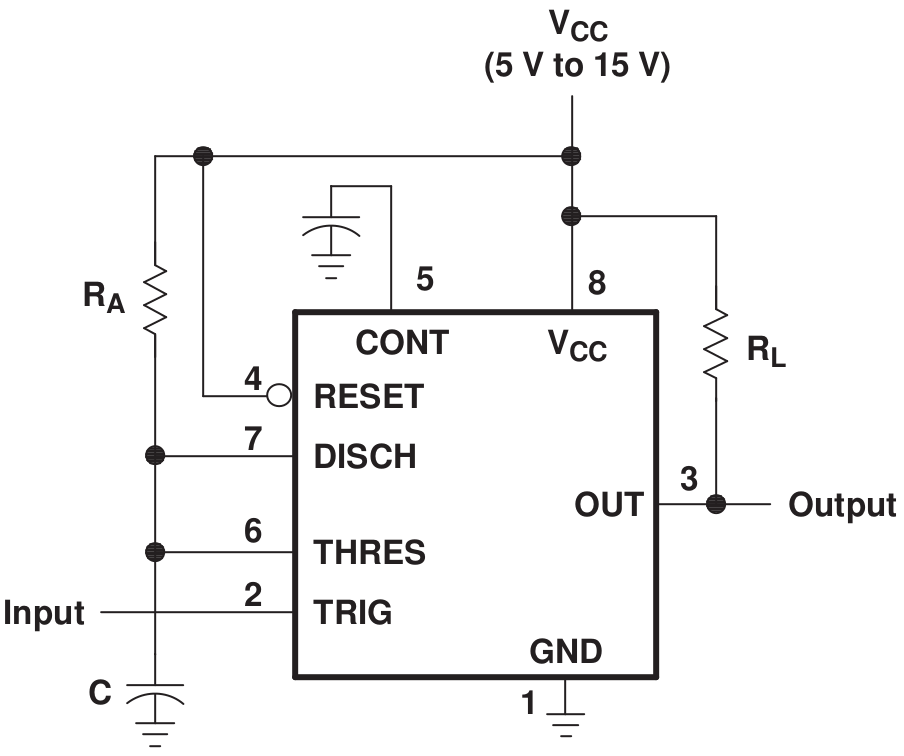
\includegraphics[width=7cm]{_fig/3d3d1_monoestable.png}
		
		donde:
		
		\[ t_w = 1.1 * R_A * C \]

		\subsubsection{Configuración Astable}

		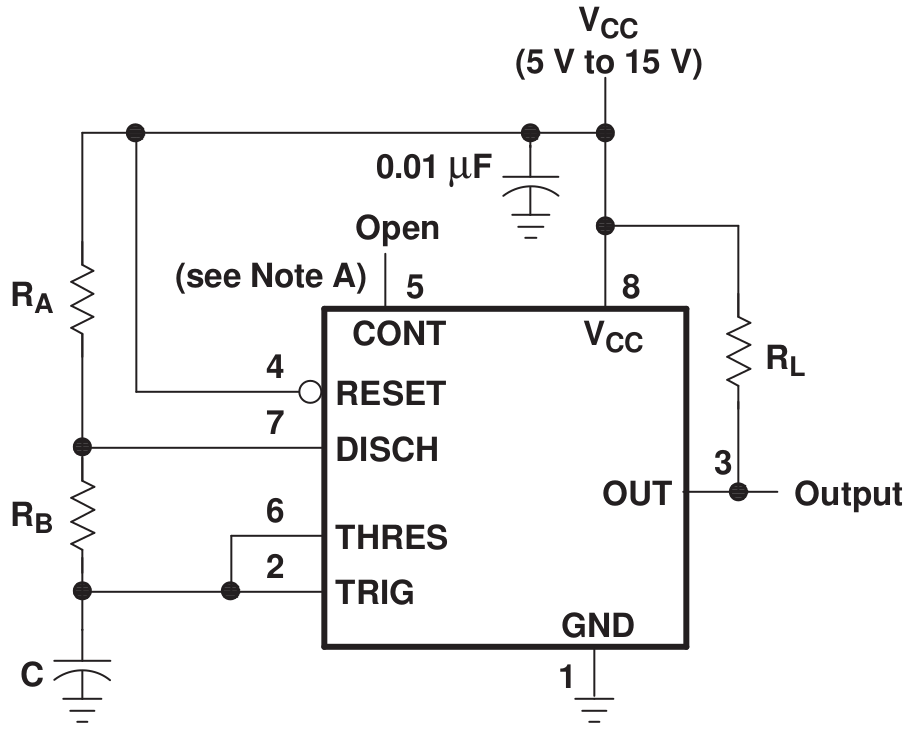
\includegraphics[width=7cm]{_fig/3d3d2_astable.png}
			
		donde:
		
		\[ t_H = 0.693 * (R_A + R_B)*C \]
		\[ t_L = 0.693 * (R_B)*C \]
		\[ T = t_H + t_L = 0.693 (R_A + 2*R_B)*C \]
		\[ f \approx \frac{1.44}{(R_A + 2*R_B)*C} \]
		\[ \frac{t_L}{t_H + t_L} = \frac{R_B}{R_A + 2*R_B} \]
		\[ \frac{t_H}{t_H + t_L} = 1 - \frac{R_B}{R_A + 2*R_B} \]
		\[ \frac{t_L}{t_H} = \frac{R_B}{R_A + R_B} \]

		\subsubsection{Configuración Secuencial}

		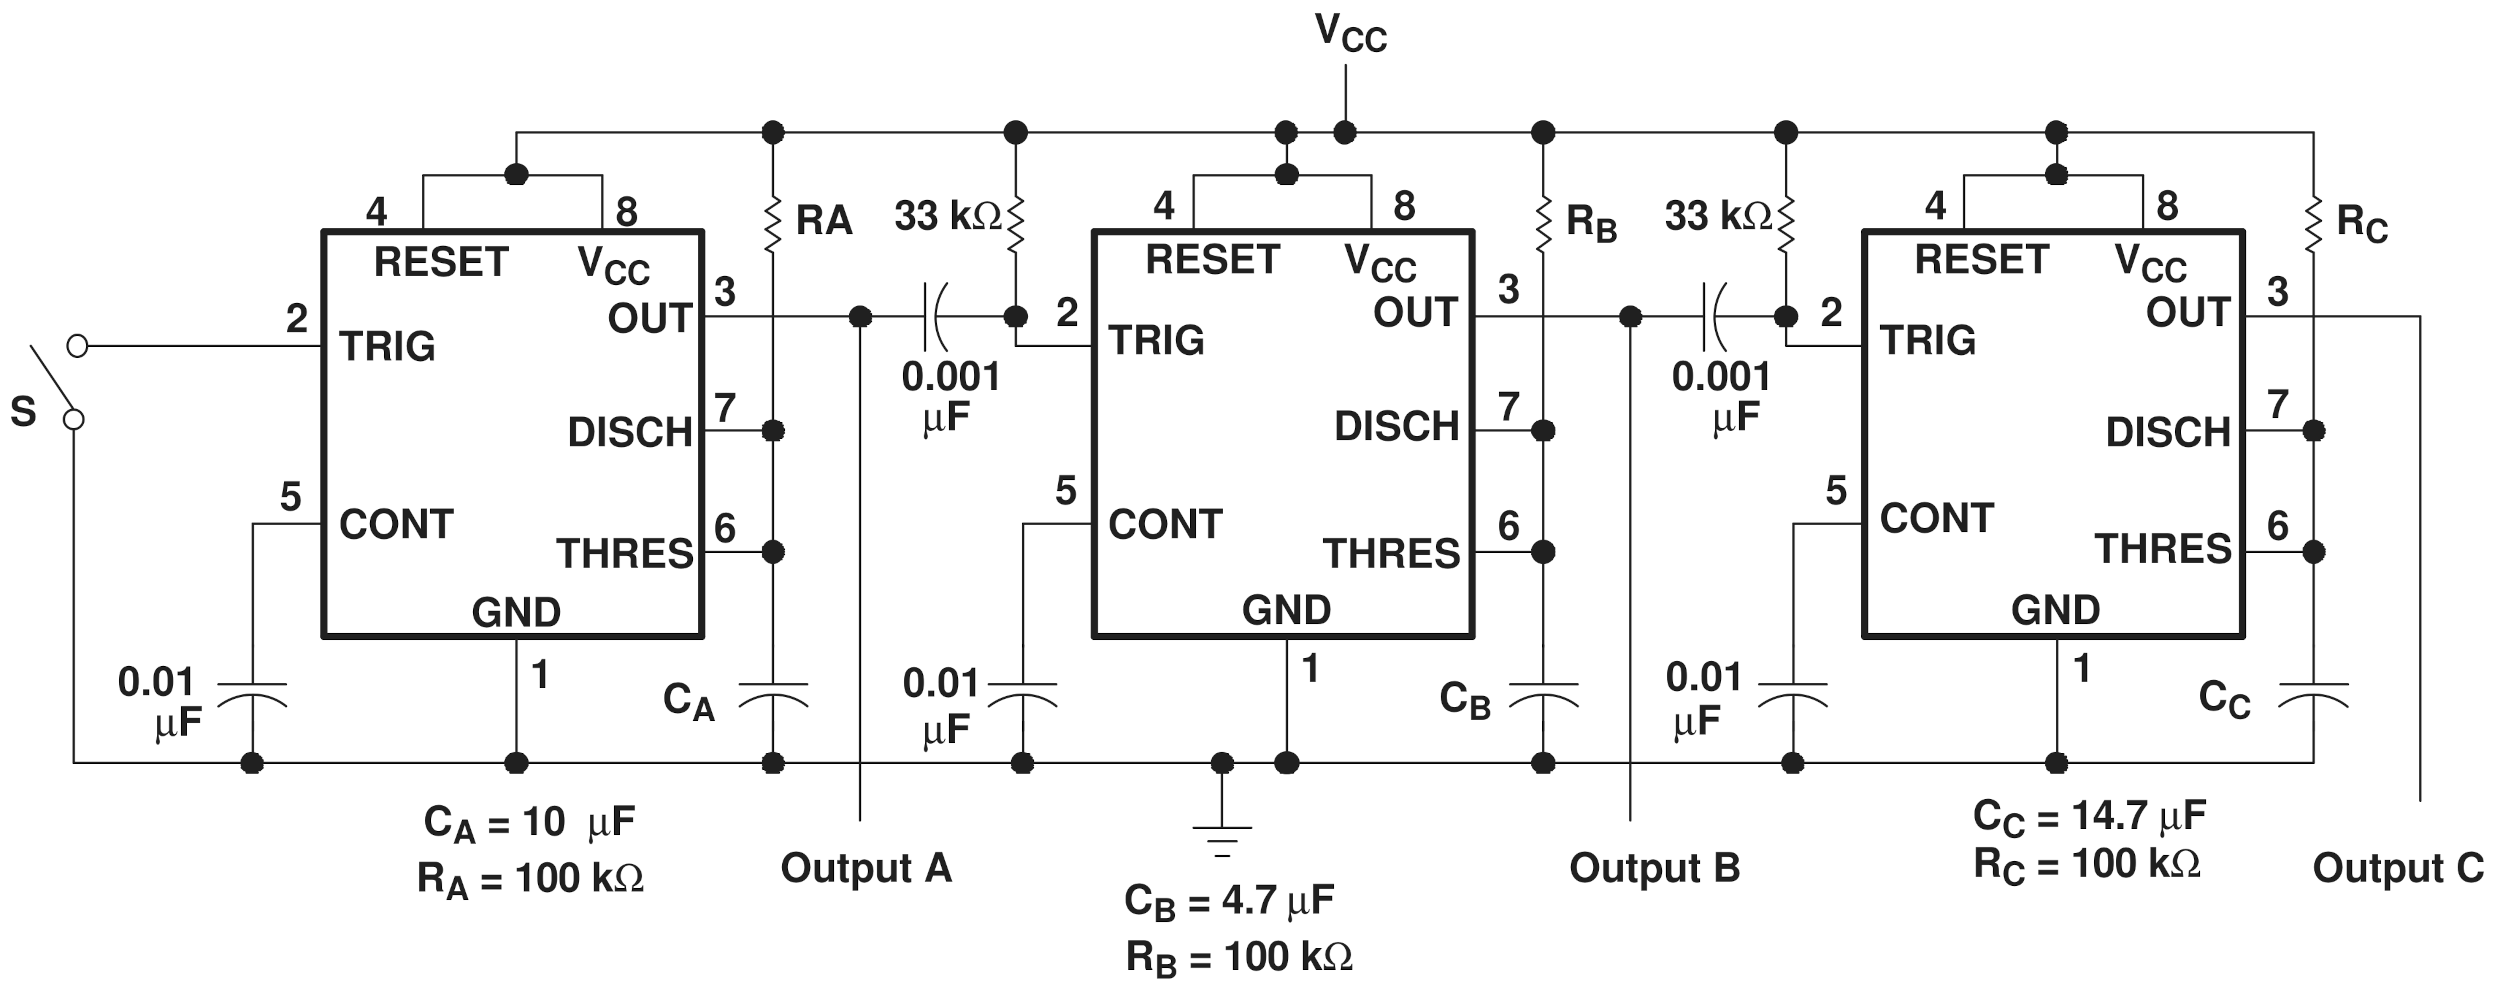
\includegraphics[width=9cm]{_fig/3d3d3_secuencial.png}
		
		Use la fórmula para configuración monoestable para calcular el $t_W$ de cada secuencia.
		
		\subsection{Generadores de rampa, diente de sierra}
		
		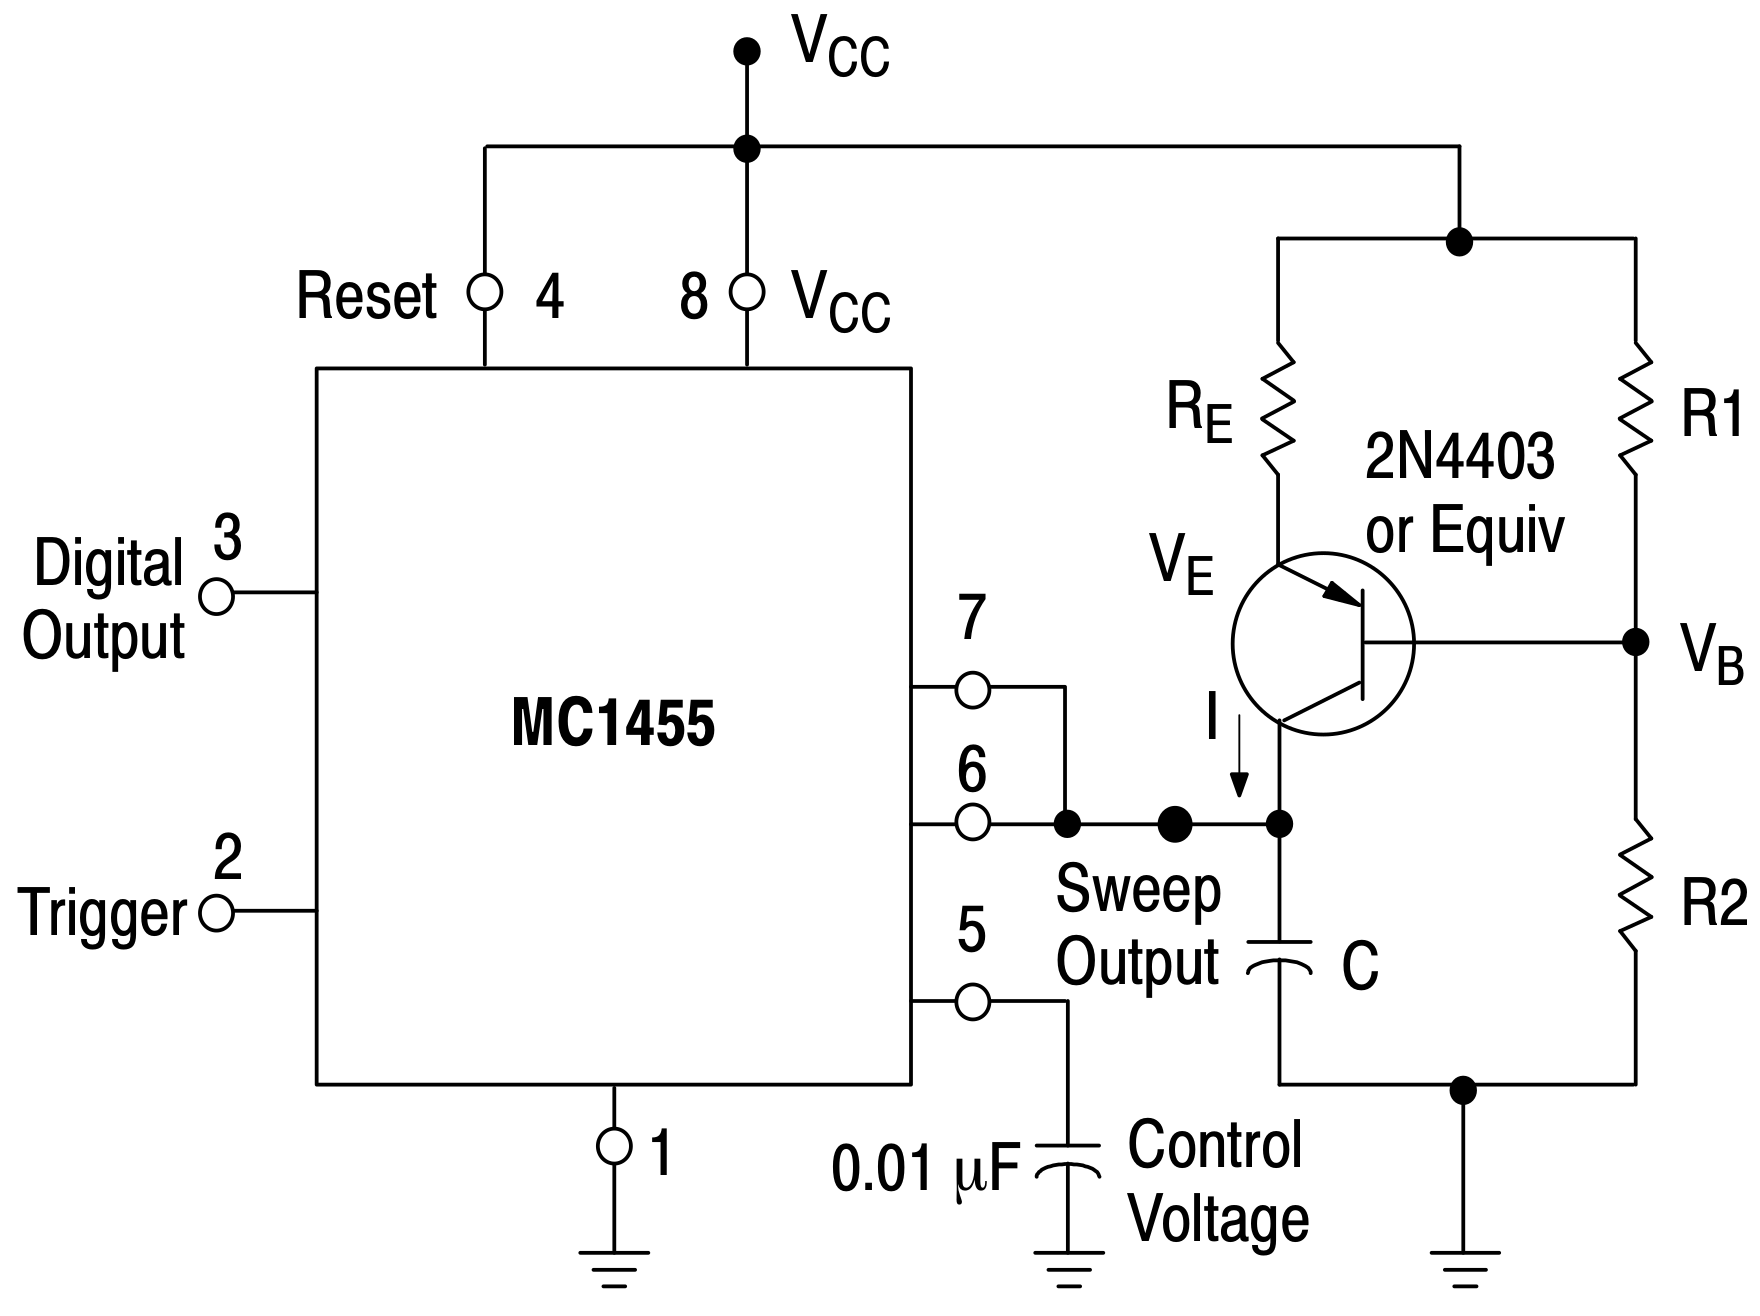
\includegraphics[width=9cm]{_fig/3d4_rampa.png}
		
		donde:
		
		\[ I = \frac{V_{CC} - V_B - V_{BE}}{R_E} \]
		\[ t = \frac{ 2/3 * V_{CC} * R_E * (R_1 + R_2) * C}{R_1 * V_{CC} - V_{BE} * (R_1 + R_2)} \]

		Más detalle ver \textit{datasheet} MC1455, \textit{Linear Voltage Ramp} en \url{https://www.onsemi.com/pdf/datasheet/mc1455-d.pdf} pag. 7.

		\subsection{Aplicaciones prácticas}
		
		

	\section{Tema IV: Familias Lógicas}
		- en desarrollo -
		\subsection{Análisis de la estructura interna de las compuertas lógicas de las familias DTL, TTL, ECL, CMOS}
		- en desarrollo -
		
		\subsection{Características de transferencia}
		- en desarrollo -
		
		\subsection{Velocidad de conmutación}
		- en desarrollo -
		
		\subsection{Fan Out}
		- en desarrollo -
		
		\subsection{Circuitos de Interfaz}
		- en desarrollo -

	\section{Tema V: Multibrivadores, Temporizadores y Generador De Funciones}
		- en desarrollo -
		\subsection{Circuitos de selección}
		- en desarrollo -
		
		\subsection{Convertidores D/A, A/D}
		- en desarrollo -
		
		\subsection{Multiplexadores analógicos}
		- en desarrollo -
		
		\subsection{Muestreador y retenedor}
		- en desarrollo -
		
		\subsection{Cálculo de errores en sistemas de adquisición de datos}
		- en desarrollo -

	\section{Recursos adicionales}
		\subsection{Espectro Electromagnético}
		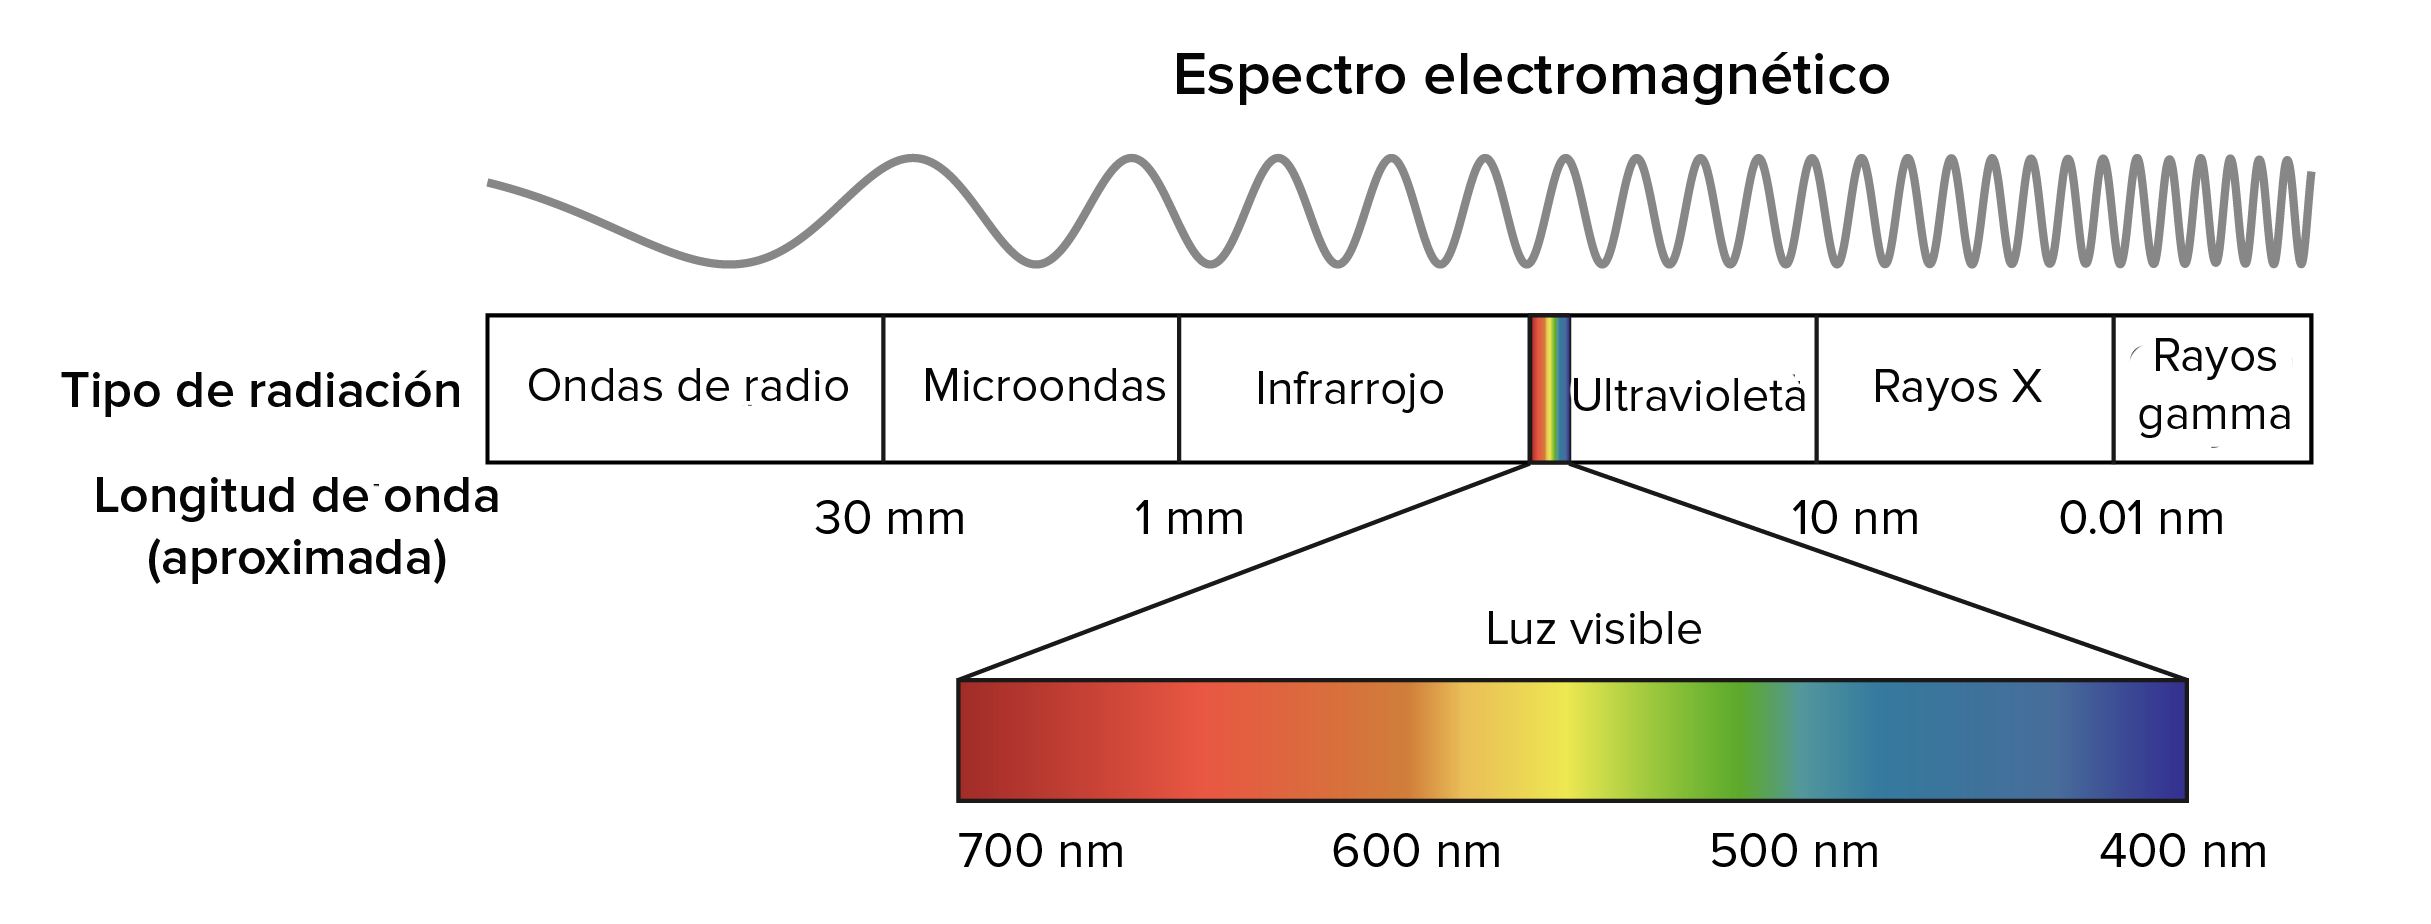
\includegraphics[width=9cm]{_fig/1d1_espectro-electromagnetico.png}

		\subsection{Ley de Ohm}
		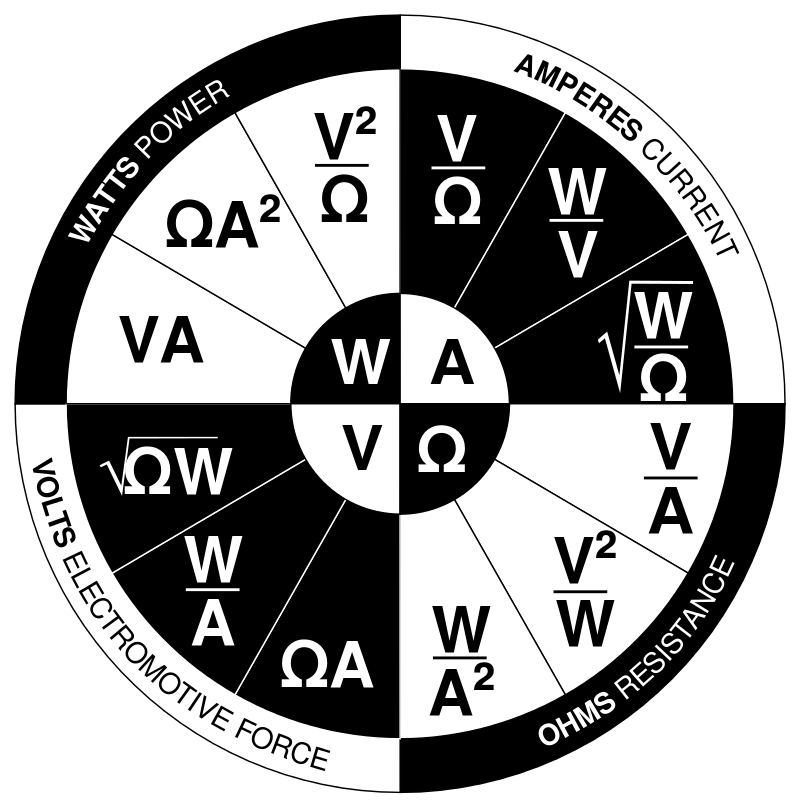
\includegraphics[width=8cm]{_fig/OhmsLaw_Wheel_WVOA.png}
		
		\subsection{Fórmulas de integrales}
		\[ \int \,dx = x + C \]
		\[ \int x^n \,dx = \frac{x^{n+1}}{n+1} + C \]
		\[ \int v^n \,dv = \frac{v^{n+1}}{n+1} + C \]
		\[ \int \frac{dv}{v} = \ln v + C \]
		\[ \int e^v \,dv = e^v + C \]
		\[ \int a^v \,dv = \frac{a^v}{\ln a} + C\]
		\[ \int \sin{v} \,dv = - \cos v + C \]
		\[ \int \cos{v} \,dv = \sin v + C \]
		\[ \int \tan{v} \,dv = - \ln{|\cos v|} + C \]
		\[ \int \cot{v} \,dv = \ln{|\sin v|} + C \]
		\[ \int \sec{v} \,dv = \ln{|\sec v + \tan v|} + C \]
		\[ \int \csc{v} \,dv = \ln{|\csc v - \cot v|} + C \]
		\[ \int \sec^2{v} \,dv = \tan{v} + C\]
		\[ \int \csc^2{v} \,dv = - \cot{v} + C\]
		\[ \int \sec{v} \cdot \tan{v} \,dv = \sec{v} + C \]
		\[ \int \csc{v} \cdot \cot{v} \,dv = - \csc{v} + C \]
		\[ \int \frac{dv}{v^2 + a^2} = \frac{1}{a} \arctan \frac{v}{a} \] 
		\[ \int \frac{dv}{v^2 - a^2} = \frac{1}{2a} \ln |\frac{v-a}{v+a}| + C \]
		\[ \int \frac{dv}{a^2 - v^2} = \frac{1}{2a} \ln |\frac{v+a}{v-a}| + C \]
		\[ \int \frac{dv}{\sqrt{v^2 \pm a^2}} = \ln{|v + \sqrt{v^2 \pm a^2}|} \]
		\[ \int \frac{dv}{\sqrt{a^2 - v^2}} = \arcsin{\frac{v}{a}} + C \]
		\[ \int \frac{dv}{v \sqrt{v^2 - a^2}} = \frac{1}{a} \arcsin{\frac{v}{a}} + C \]
		\[ \int \sqrt{v^2 \pm a^2}\ dv = \frac{v}{2} \sqrt{v^2 \pm a^2} \pm \frac{a^2}{2} \ln{|v + \sqrt{v^2 \pm a^2}|} + C \]
		\[ \int \sqrt{a^2 - v^2}\ dv = \frac{v}{2} \sqrt{v^2 - a^2} + \frac{a^2}{2} \arcsin{\frac{v}{a}} + C \]
		
		\subsection{Fórmulas de derivadas}
		\[ \frac{\partial}{\partial x}\ c = 0 \]
		\[ \frac{\partial}{\partial x}\ x = 1 \]
		\[ \frac{\partial}{\partial x}\ cx = c \]
		%		\[ \frac{\partial}{\partial x}\ x^n = nx^{n-1} \]
		\[ \frac{\partial}{\partial x}\ v^n = nv^{n-1} \frac{\partial v}{\partial x} \]
		\[ \frac{\partial}{\partial x}\ uv = \frac{\partial u}{\partial x}v + u\frac{\partial v}{\partial x} \]	
		\[ \frac{\partial}{\partial x} \frac{u}{v} = \frac{v\frac{\partial u}{\partial x}-u\frac{\partial v}{\partial x}}{v^2} \]
		\[ \frac{\partial}{\partial x}\ ln{\ v} = \frac{\frac{\partial}{\partial x}v}{v} \]
		\[ \frac{\partial}{\partial x}\ log{_{a}v} = \frac{log{_{a}e}}{v}\frac{\partial v}{\partial x} \]
		\[ \frac{\partial}{\partial x} e^v = e^v\frac{\partial v}{\partial x} \]
		\[ \frac{\partial}{\partial x} a^v = a^v\ ln{\ a}\frac{\partial v}{\partial x} \]
		\[ \frac{\partial}{\partial x} u^v = v\ u^{v-1}\frac{\partial u}{\partial x} + u^v\ ln{\ u}\frac{\partial v}{\partial x} \]
		\[ \frac{\partial}{\partial x} \sin{v} = \cos{v}\frac{\partial v}{\partial x} \]
		\[ \frac{\partial}{\partial x} \cos{v} = -\sin{v}\frac{\partial v}{\partial x} \]
		\[ \frac{\partial}{\partial x} \tan{v} = \sec^2{v}\frac{\partial v}{\partial x} \]
		\[ \frac{\partial}{\partial x} \cot{v} = -\csc^2{v}\frac{\partial v}{\partial x} \]
		\[ \frac{\partial}{\partial x} \sec{v} = \sec{v}\tan{v}\frac{\partial v}{\partial x} \]
		\[ \frac{\partial}{\partial x} \csc{v} = -\csc{v}\cot{v}\frac{\partial v}{\partial x} \]
		\[ \frac{\partial}{\partial x} \arcsin{v} = \frac{\frac{\partial v}{\partial x}}{\sqrt{1-v^2}} \]
		\[ \frac{\partial}{\partial x} \arccos{v} = \frac{-\frac{\partial v}{\partial x}}{\sqrt{1-v^2}} \]
		\[ \frac{\partial}{\partial x} \arctan{v} = \frac{\frac{\partial v}{\partial x}}{1+v^2} \]
		
		\subsection{Fórmulas de transformada de Laplace}
		\[ 1 = \frac{1}{S} \]
		\[ t = \frac{1}{S^2} \]
		\[ e^{at} = \frac{1}{S-a} \]
		\[ \sin(\omega t) = \frac{\omega}{S^2+\omega^2} \]
		\[ \cos(\omega t) = \frac{S}{S^2+\omega^2} \]
		\[ \sinh(\omega t) = \frac{\omega}{S^2-\omega^2} \]
		\[ \cosh(\omega t) = \frac{S}{S^2-\omega^2} \]
		\[ \frac{\partial f}{\partial t} = f'{(t)} = SF(S)-F(0) \]
		\[ \frac{\partial^2 f}{\partial t^2} = f''{(t)} = S^2F(S)-SF(S) - F'(0) \]
		\[ \int f(t) \,dt = \frac{F(S)}{S} \]
		\[ t^n \,(n=1,2,3, ...) = \frac{n!}{S^{n+1}} \]
		\[ t^n e^{at} = \frac{n!}{{(S-a)}^{n+1}} \]
		\[ t \sin(\omega t) = \frac{2 \omega S}{{(S^2+\omega^2)}^2} \]
		\[ t \cos(\omega t) = \frac{S^2-\omega^2}{{(S^2+\omega^2)}^2} \]
		\[ e^{at} \sin(\omega t) = \frac{\omega}{{(S-a)}^2+\omega^2} \]
		\[ e^{at} \cos(\omega t) = \frac{S-a}{{(S-a)}^2+\omega^2} \]

	\section{Operaciones básicas}
		\subsection{Integración}
		Es una generalización de la suma de infinitos sumandos, infinitesimalmente pequeños: una suma continua. La integral es la operación inversa a la diferencial de una función, como se observa en la figura:
		
		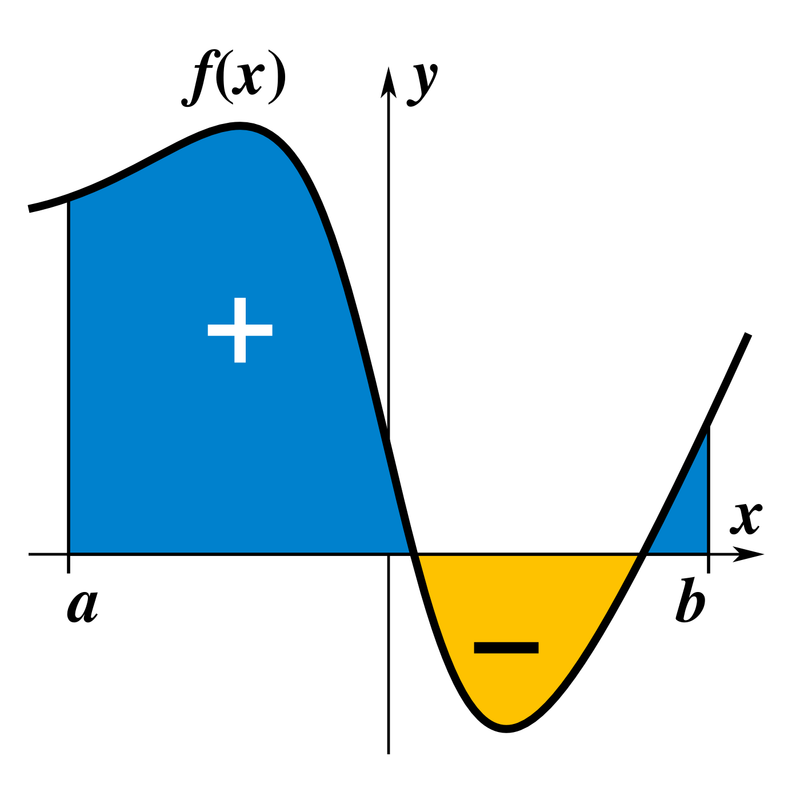
\includegraphics[width=7cm]{_fig/Integral_Example.png}
		
		\subsubsection{Ejemplo de integrales}
		\[ \int e^{2x} \,dx \]
		
		Para ésto aplicamos por método de sustitución, tenemos:
		
		\[ \begin{matrix}
			u=2x \\
			du = 2dx \\
			\frac{du}{2} = dx
		\end{matrix} \]
		
		\[ \int e^{2x} \,dx = \int e^{u} \,\frac{du}{2} = \frac{1}{2}\int e^{u} \,du = \frac{1}{2} e^{u} + C = \frac{1}{2} e^{2x} + C\]
	
		\subsection{Transformada de Laplace}
		Es un método que nos permite resolver ecuaciones diferenciales \textit{"en resumen"}, y para entender dicha operación es necesario tener claro la solución de lo siguiente: 
		
		1. La solución de una \textbf{integral definida}, asumamos el siguiente ejemplo:
		
		\[ \int_{1}^{2} xy \,dx = \frac{1}{2}x^2y \bigg\rvert_{1}^{2} = \frac{3}{2}y \]
		
		Una de las variables "desaparece" al ser evaluada en los limites de la integración, como resultado nos queda una función de \(y\).
		
		2. La solución de una \textbf{integral impropia}, asumamos el siguiente ejemplo:
		
		\[ \int_{1}^{\infty} \frac{dx}{x^2} = -\frac{1}{x} \bigg\rvert_{1}^{\infty} = -\lim_{x\to\infty}(\frac{1}{x}) + \frac{1}{1} = 0 + 1 = 1 \]
		
		%% cuando da un valor numerico se dice que "converge" de lo contrario "diverge"
		
		Entonces dado esto decimos que la transformada de Laplace es como sigue:
		
		\[ \mathscr{L}{f(t)} = \int_{0}^{\infty} f(t)e^{-st} \,dt \]
		
		Por lo que es una integral de dos variables (\(s\) y \(t\)), se está integrando respecto de \(t\) lo que significa que \(s\) es una constante, cuando integremos y evaluemos en los límites de integración resulta una función de \(t\)
		
		\subsubsection{Ejemplo de Transformada de Laplace}
		\[ \mathscr{L}{[1]} = \int_{0}^{\infty} e^{-st} \,dt = -\frac{1}{s} e^{-st} \bigg\rvert_{0}^{\infty} = -\lim_{t\to\infty}\frac{1}{s} e^{-st} + \frac{1}{s} e^{-s(0)} \]
		\[ \mathscr{L}{[1]} = -\frac{1}{s} \lim_{t\to\infty} e^{-st} + \frac{1}{s} \]
		
		%% El limite va a depender del valor de s
		
		analizando el (\(\lim\)) y sus posibles casos tenemos:
		
		\[ \lim_{x\to\infty} e^{kx} = \begin{Bmatrix}
			0, si & k<0 \\
			1, si & k=0 \\
			\infty, si & k>0
		\end{Bmatrix} \]		
		
		%% Nosotros queremos que este resultado "convergue" por lo que no interesa el valor infty, tenemos 0,si y 1,si, 1,si o k=0 no es posible porque al colocar k=0 o s=0 tendriamos divisiones entre 0, solo nos queda 0,si para k<0
		
		\[  \mathscr{L}{[1]} = \frac{1}{s} \,\,\,\, (s>0) \]
		
		% No hace falta colocar el dominio (s>0) normalmente cuando resolvamos ecuaciones diferenciales (o transformada de laplace), en adelante solo basta con colocar 1/s

\end{document}
